\chapter{Útkereső algoritmus}

A hexagonok és a négyzetek esetén az útkeresés csak egy ponton különbözik (szomszédok száma) ezért az egyszerűség kedvért csak a négyzethálónál mutatom be.
\newline
\newline Az algoritmus:
\begin{verbatim}
OPEN //the set of nodes to be evaluated
CLOSED //the set of nodes already evaluated
add the start node to OPEN

loop
  current = node in OPEN  with the lowest f_cost
  remove current from OPEN
  add current to CLOSED

  if current is the target node //path has been found
    return

  foreach neighbour of the current node
    if neighbour is not traversable or neighbour is in CLOSED
      skip to the next neighbour

    if new path to neighbour is shorter OR neighbour is not in OPEN
      set f_cost of neighbour
      set parent of neighbour to current
      if neighbour is not in OPEN
        add neighbour to OPEN
\end{verbatim}

\section{Szomszédok}

Ahhoz, hogy útkereső algoritmust tudjunk készíteni ismernünk kell, hogy a különböző alakzatok és koordináta rendszerek esetén milyen algoritmussal érhetjük el az adott alakzat szomszédait. 
\newline
\newline Az algoritmusokat ebben a formában fogom megadni: $A \rightarrow B1, B2, B3 …$
(Az $''A''$ és $''B''$ pontokat $''u''$, $''v''$ koordináták segítségével fogom megadni.)

\subsection{Négyzet}
A négyzet esetén egyszerű dolgunk van, mert csak egyfajta koordináta rendszerünk van.

$$
(u,v) \rightarrow (u,v+1) (u+1,v) (u,v-1), (u-1,v)
$$

\subsection{Hexagon}

Hexagon esetén több fajta koordináta rendszerünk is lehet.

\subsubsection{Kocka koordináta rendszer (Cube coordinates)}

\noindent Ahhoz, hogy elmozduljunk eggyel meg kell változtatnunk egyet a három kocka koordináta közül $+1$-el és egy másikat $-1$-el (a változtatások összege $0$ kell, hogy legyen). Három koordinátát lehet megváltoztatni $+1$-el, a másik két lehetséges koordináta közül az egyiket kell csökkenteni $-1$-el. Ez hat lehetséges változatot eredményez. Mindegyik megfeleltethető a hexagon egyik irányának. A lehető legegyszerűbb és leggyorsabb megoldás az, ha az összes lehetséges permutációt előre kikalkuláljuk és beleírjuk egy táblázatba ( Cube($dx, dy, dz$)).
\newline
\newline Algoritmus: 
\begin{verbatim}
var cube_directions = [
   Cube(+1, -1,  0), Cube(+1,  0, -1), Cube( 0, +1, -1),
   Cube(-1, +1,  0), Cube(-1,  0, +1), Cube( 0, -1, +1)
]

function cube_direction(direction):
    return cube_directions[direction]

function cube_neighbor(cube, direction):
    return cube_add(cube, cube_direction(direction))
\end{verbatim}

\subsubsection{Tengely koordináta rendszer (Axial coordinates)}

\noindent A kocka koordináta rendszer veszük alapul. Mégpedig úgy, hogy a Cube($ dx, dy, dz$) koordinátákat átalakitjuk Axial($ dx, dz$) -re.
\newline
\newline Algoritmus:
\begin{verbatim}
var axial_directions = [
   Hex(+1,  0), Hex(+1, -1), Hex( 0, -1),
   Hex(-1,  0), Hex(-1, +1), Hex( 0, +1)
]

function hex_direction(direction):
    return axial_directions[direction]

function hex_neighbor(hex, direction):
    var dir = hex_direction(direction)
    return Hex(hex.q + dir.q, hex.r + dir.r)
\end{verbatim}

\subsubsection{Eltolásos koordináta rendszer (Offset coordinates)}

\noindent Eltolásos koordináta rendszer esetén a lépések változnak annak a függvényében, hogy hol állunk a hálóban. Ha mi egy eltolt oszlopban/sorban állunk akkor a szabály eltér attól mintha egy nem eltolt oszlopban/sorban állnánk.
\newline
\newline Ahogy a korábbi esetekben úgy most is kell készítenünk egy táblázatot amiben azt tároljuk majd, hogy a különböző tengelyeken mennyit kell hozzáadni, hogy elérjük a szomszédokat. De ebben az esetben most két tömbre lesz szükségünk, az egyik a páros sor/oszlop a másik pedig a páratlan sor/oszlop esetére.
\newline
\newline A táblázat különbözik mind a négy eltolásos módszernél.
\newline
\newline Páratlan sor: 
\begin{verbatim}
var oddr_directions = [
   [ Hex(+1,  0), Hex( 0, -1), Hex(-1, -1),
     Hex(-1,  0), Hex(-1, +1), Hex( 0, +1) ],
   [ Hex(+1,  0), Hex(+1, -1), Hex( 0, -1),
     Hex(-1,  0), Hex( 0, +1), Hex(+1, +1) ]
]

function oddr_offset_neighbor(hex, direction):
    var parity = hex.row & 1
    var dir = oddr_directions[parity][direction]
    return Hex(hex.col + dir.col, hex.row + dir.row)
\end{verbatim}
Páros sor: 
\begin{verbatim}
var evenr_directions = [
   [ Hex(+1,  0), Hex(+1, -1), Hex( 0, -1),
     Hex(-1,  0), Hex( 0, +1), Hex(+1, +1) ],
   [ Hex(+1,  0), Hex( 0, -1), Hex(-1, -1),
     Hex(-1,  0), Hex(-1, +1), Hex( 0, +1) ]
]

function evenr_offset_neighbor(hex, direction):
    var parity = hex.row & 1
    var dir = evenr_directions[parity][direction]
    return Hex(hex.col + dir.col, hex.row + dir.row)
\end{verbatim}
Páratlan oszlop: 
\begin{verbatim}
var oddq_directions = [
   [ Hex(+1,  0), Hex(+1, -1), Hex( 0, -1),
     Hex(-1, -1), Hex(-1,  0), Hex( 0, +1) ],
   [ Hex(+1, +1), Hex(+1,  0), Hex( 0, -1),
     Hex(-1,  0), Hex(-1, +1), Hex( 0, +1) ]
]

function oddq_offset_neighbor(hex, direction):
    var parity = hex.col & 1
    var dir = oddq_directions[parity][direction]
    return Hex(hex.col + dir.col, hex.row + dir.row)
\end{verbatim}
Páros oszlop: 
\begin{verbatim}
var evenq_directions = [
   [ Hex(+1, +1), Hex(+1,  0), Hex( 0, -1),
     Hex(-1,  0), Hex(-1, +1), Hex( 0, +1) ],
   [ Hex(+1,  0), Hex(+1, -1), Hex( 0, -1),
     Hex(-1, -1), Hex(-1,  0), Hex( 0, +1) ]
]

function evenq_offset_neighbor(hex, direction):
    var parity = hex.col & 1
    var dir = evenq_directions[parity][direction]
    return Hex(hex.col + dir.col, hex.row + dir.row)
\end{verbatim}

\subsubsection{Átlós szomszédok}

\noindent Az “átlós” szomszédok a kocka koordináták esetén úgy működik, hogy a lehetséges három koordináta közül az egyiket $ \pm 2$ -vel, míg a másik kettőt $\mp 1$ -el módosítjuk, hogy a három koordináta összege mindig $0$ legyen.

\begin{figure}[h]
\centering
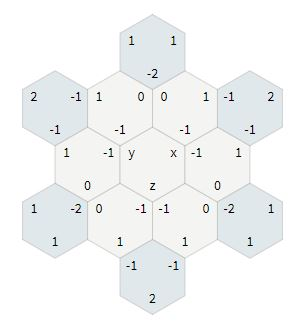
\includegraphics[scale=0.4]{kepek/img81.JPG}
\caption{"Átlós" szomszédok}
\label{fig:img81}
\end{figure}

\noindent Algoritmus:
\begin{verbatim}
var cube_diagonals = [
   Cube(+2, -1, -1), Cube(+1, +1, -2), Cube(-1, +2, -1), 
   Cube(-2, +1, +1), Cube(-1, -1, +2), Cube(+1, -2, +1)
]

function cube_diagonal_neighbor(cube, direction):
    return cube_add(cube, cube_diagonals[direction])
\end{verbatim}

\noindent Tengelyes koordináta rendszer használta esetén is lehetséges az algoritmus használta.
